\documentclass[border={0.1cm 0.1cm 0.1cm -1.25cm}]{standalone}  %E,S,W,N
%\documentclass{scrartcl}

\usepackage{amssymb}
\usepackage{amsmath}
\usepackage{graphicx}
\usepackage{tikz}
\usetikzlibrary{shapes} %for node shapes
\usetikzlibrary{calc}	%for centerarc

\begin{document}
	
	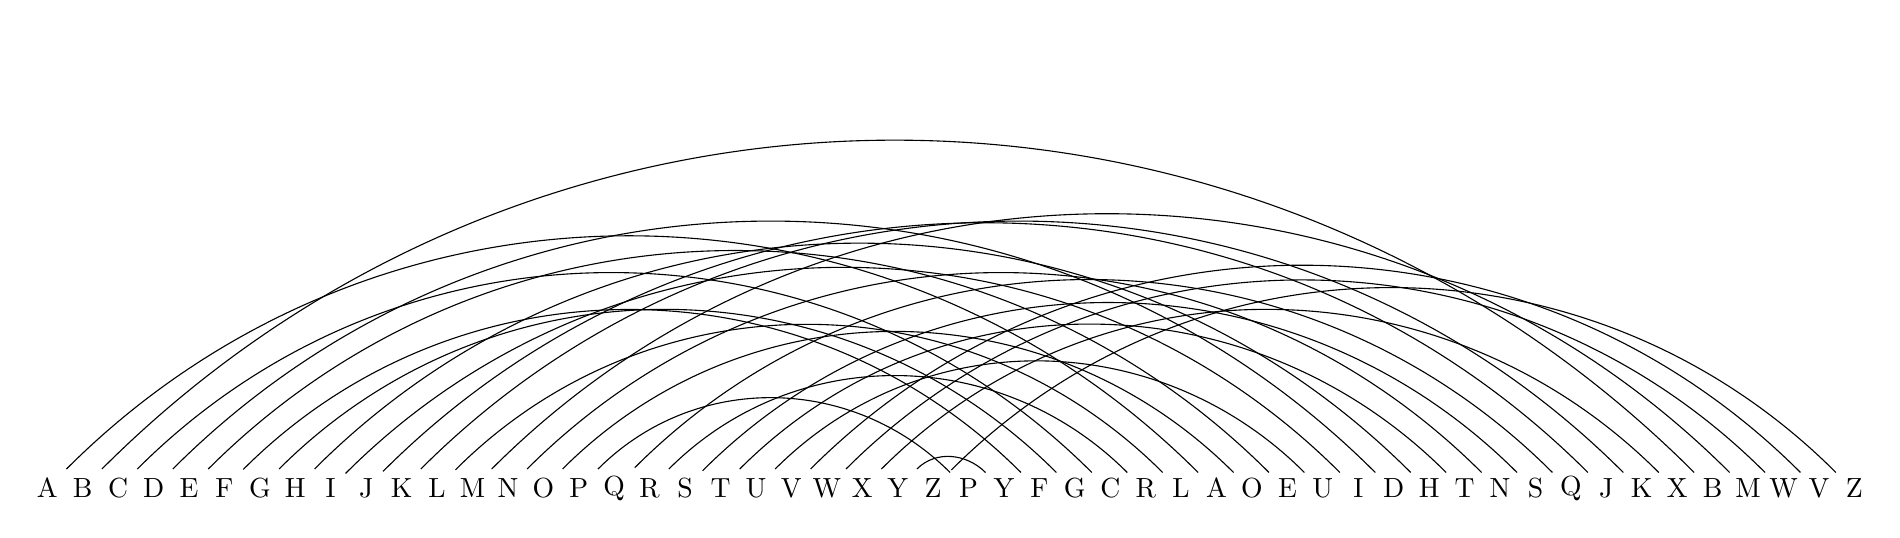
\begin{tikzpicture}	
	\def\s{0.45}	
	\foreach \i [count=\j] in {A,...,Z} \node (\i) at (\s*\j,0) {\i};
	\foreach \i [count=\j] in {P,Y,F,G,C,R,L,A,O,E,U,I,D,H,T,N,S,Q,J,K,X,B,M,W,V,Z}{
		\node at ({26*\s+\s*\j},0) {\i};
		\draw[xshift=\s] ({26*\s+\s*\j-0.25},0.2) to[out=135,in=45] (\i);
	}
	\end{tikzpicture}
	
\end{document}